%!TEX root = thesis.tex

\section{Small Boat Fleet and Shipping Decarbonisation}
Current literature related to estimating small-scale vessels without machine learning methods includes using statistical factors or measures.~\newcite{johnson2017spatial} used Kernel Density Estimation (KDE) to distribute data on the population, the number of ships, and the average annual total catch for the entire population, and finally showed that their forecasts could accurately predict the landing of fisheries in the bay. In their paper, they explained the source of their data~\cite{Lopez-Sagastegui2017Comparing}. Lopez-Sagastegui et al. worked with fishermen to generate and record information about fish catches, fishing effort, profits, species breeding seasons, and spatial patterns of fishing activities. However, one of the points to make against this work is that it only focuses on fishing vessels. While these are the majority, it still misses the other ship types. Notably, the authors provided information (Figure~\ref{review_density_of_gulf}) of the density of human population and boats in the Gulf of California that can save much time in creating data sets of the Gulf of California for training machines learning models.\\

\begin{figure}[t]
\center
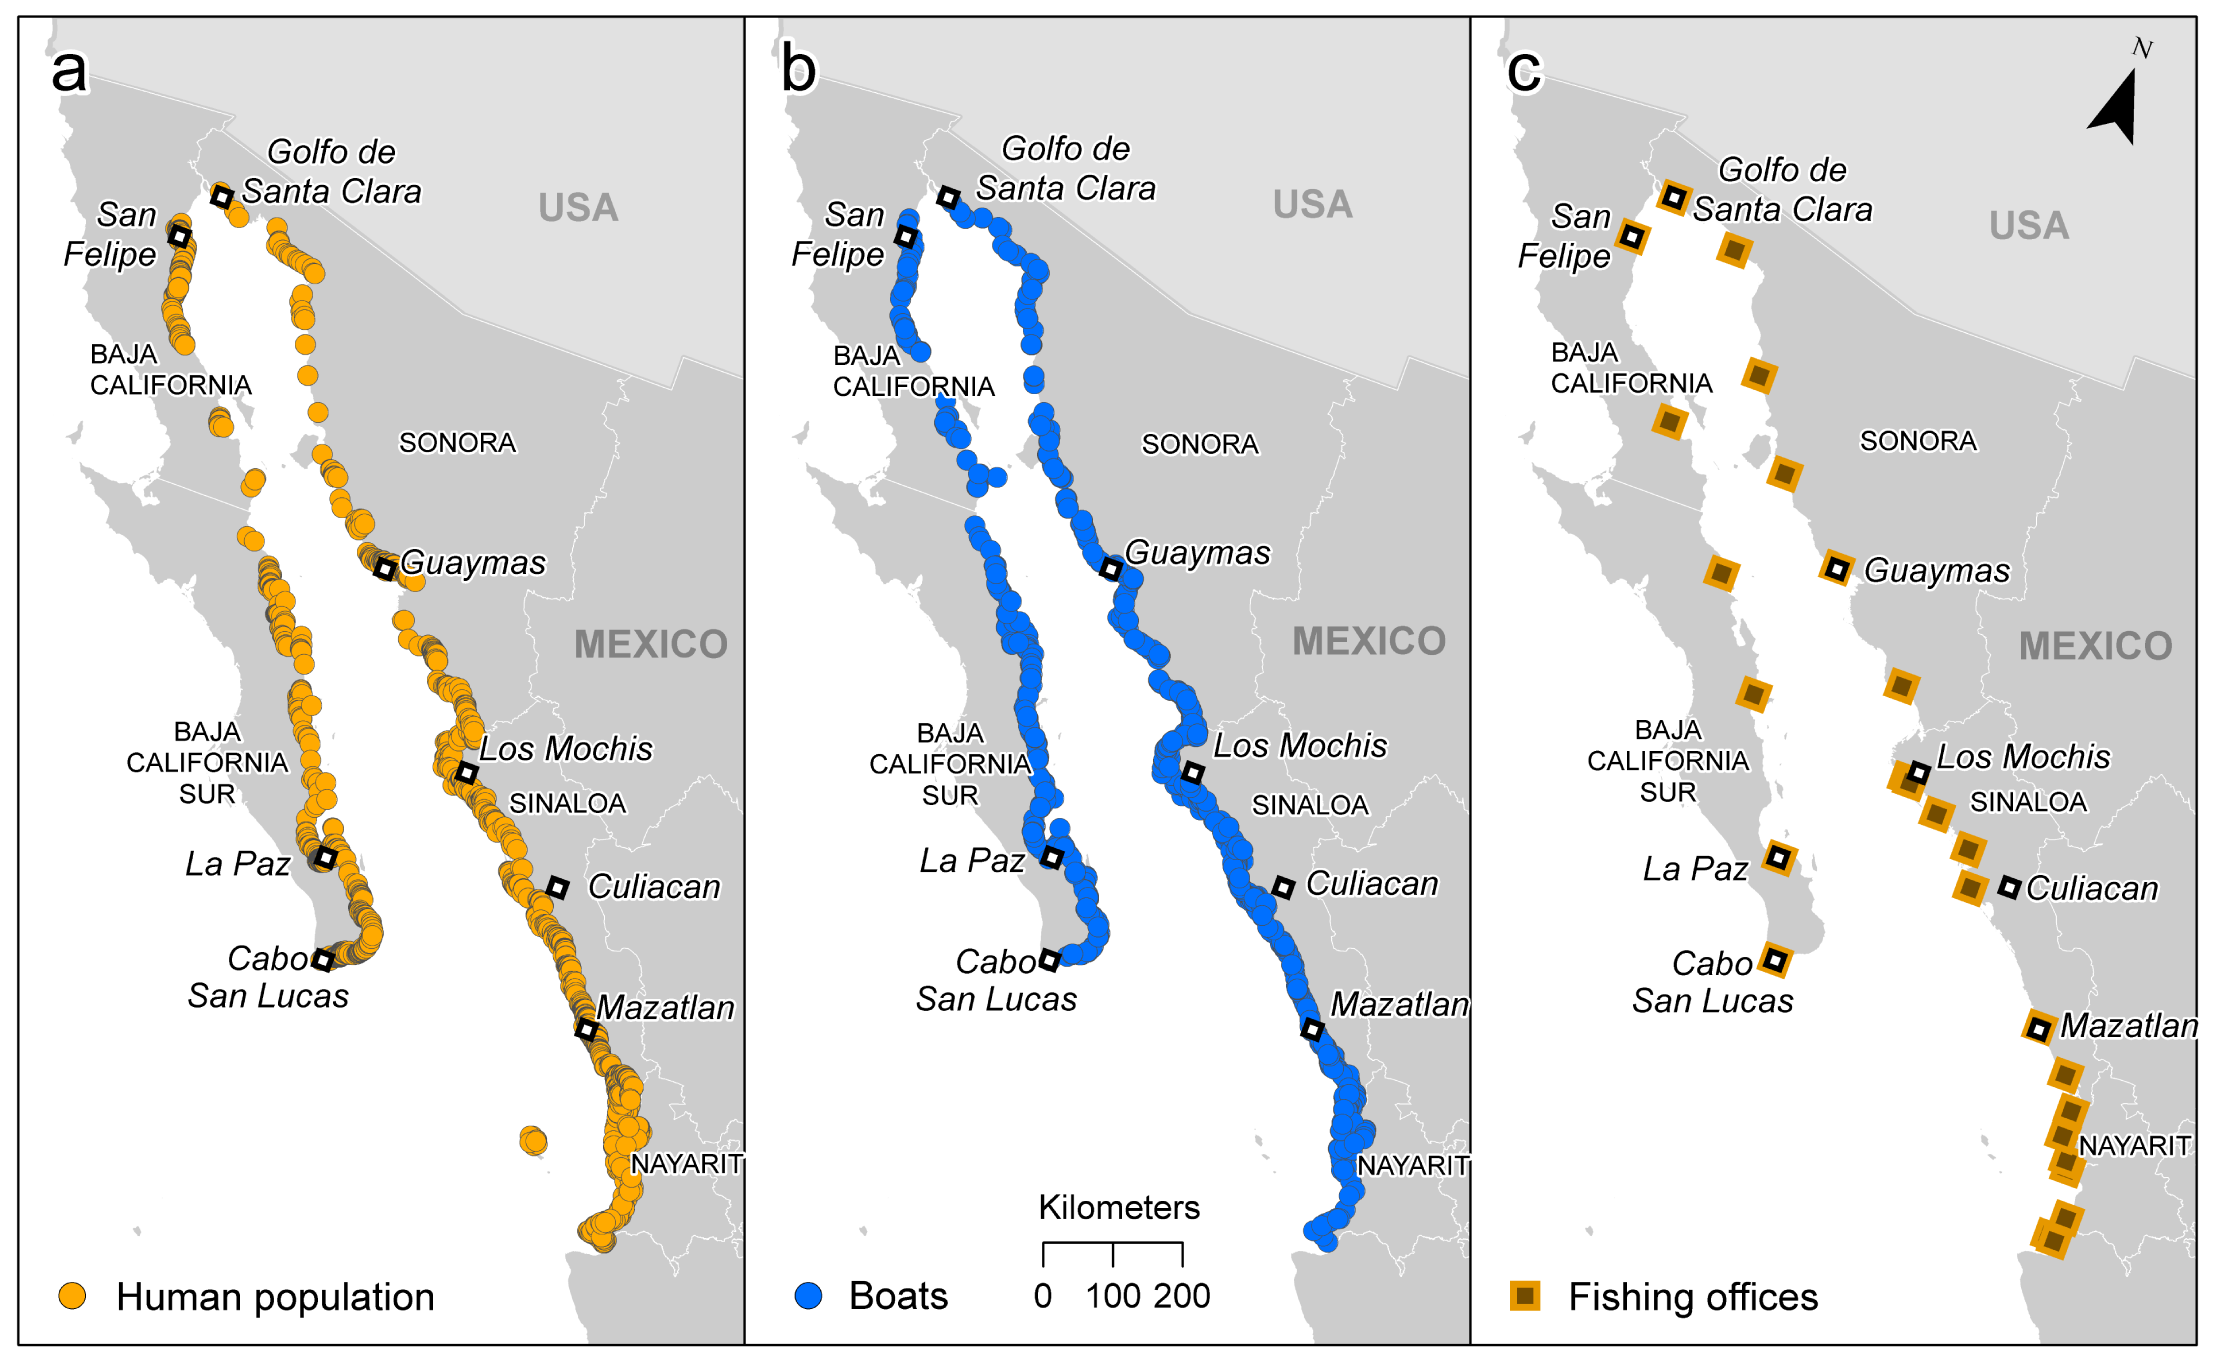
\includegraphics[scale=0.83]{img/review_density_of_gulf.png}
\longcaption{Map of the density of human population, boats, and fishing offices in the Gulf of California.}{\label{review_density_of_gulf} Map of the density of human population, boats, and fishing offices in the Gulf of California. Image courtesy: https://doi.org/10.1371/journal.pone.0174064.g002}
\end{figure}

~\newcite{Johansson2018ModelingOL} proposed a new model (FMI-BEAM) to describe the emissions of the leisure boat fleet in the Baltic Sea region with over 3000 dock locations, national small boat registry, AIS data and vessel survey results. However, the method cannot cover countries with no national registry for small boats. Besides, small boats are not just leisure boats.~\newcite{Ug2020EstimationOW} estimated global ship emissions with the help of data from the Automatic Identification System (AIS). They set up movement information relating to ship size and speed and meteorological and marine environmental conditions. Over 3,000,000,000 daily AIS data records from hundreds of owners and thousands of partner AIS base stations and detailed ship data. However, this method is highly dependent on AIS data which is impossible for unregistered small boats.~\newcite{Traut2013MonitoringSE, Johansson2016ACM, Mabunda2014EstimatingCD, Hensel2020GreenSU, Han2016RealtimeIA} have proposed the use of AIS to monitor the carbon emissions of the fleet as well.\\

~\newcite{Zhang2019TheSO} included unidentified vessels in the AIS-based vessel emission inventory. They developed an AIS-instrumented emissions inventory, including both identified and unidentified vessels. In particular, missing vessel parameters for unidentified vessels were estimated from a classification regression of vessels with similar vessel types and sizes in the AIS database. However, the authors do not discuss whether the regression model applies to vessels in most coastal areas of the planet. In addition, the authors do not discuss whether the vessel data in the AIS database is regionally diverse. Finally, if there is a diversity of vessels in the AIS database, the authors did not discuss whether this diversity would produce more significant errors in the predictions for small vessels in a single region (e.g. the Gulf of California, Mexico).


\section{Convolutional Neural Networks in Image Recognition}
Literature tends to be inaccurate for emission inventories for the small boat fleet. The above literature review has demonstrated that there is still a lot of work to do in order to understand how the small boat fleet is being operated, what fuels they are using and the level of activity for this shipping sector. This master thesis project intends to use image recognition algorithms for the identification of small boats in any sea area, significantly reducing the time taken to calculate small vessel emission inventories. Besides, it will be in the national interest for the small fleet to account for and control these emissions within the powers of the state, incentivising the energy-efficient technologies and fuel change. Further, if countries are to meet their ambitious net-zero carbon emissions targets, they cannot afford to ignore the small boat fleet emission inventories that can help governments account for carbon emissions from small boats more quickly.\\

Object detection is an active topic in image recognition and computer vision. In the past few years, this topic has made significant progress. With the rise of self-driving cars and face detection, there is an increasing demand for fast and accurate objects detection. In 2012, AlexNet won the ImageNet Large-Scale Visual Recognition Challenge (ILSVRC), making convolutional neural networks the dominant mode of image recognition~\cite{krizhevsky2012imagenet}. Then,~\newcite{girshick2014rich} introduced R-CNN, which is the first CNN-based object detection method, but with higher performance.\\

Unlike other deep learning problems, the unknown number, size and categories of instances in each image in the object detection problem lead to unexplored dimensions of the model output. Therefore, it is not easy to adapt the classic deep learning classification model that expects a fixed output size to the object detection problem. Region-Based Convolutional Neural Networks (R-CNN) may be the way to meet this challenge.\\

Since its inception, Region-Based Convolutional Neural Networks (R-CNN) has gone through many iterations: R-CNN, Fast R-CNN, Faster R-CNN and Mask R-CNN~\cite{girshick2014rich, girshick2015fast, ren2015faster, he2017mask}. To avoid computationally expensive, pixel-level classification and object search, the original R-CNN method applied a non-deep learning algorithm called Selective Search to obtain approximately 2000 region suggestions~\cite{uijlings2013selective, girshick2014rich}. Then, with the help of a modified version of the AlexNet model, features are extracted from the proposed region. The objects in the image have different scales and sizes, so their corresponding image crops need to be warped to fit the following CNN input size. Then, the support vector machine (SVM) classifier uses the extracted features for classification, and the linear regression predicts the offset of the bounding box, thereby tightening the bounding box around the object~\cite{girshick2014rich}.\\

R-CNN is an intuitive architecture that has achieved high accuracy in object detection. However, since the reasoning time for each image is about 30 seconds, this model is very inefficient for applications that require real-time prediction~\cite{huang2017speed}. Fast R-CNN performs feature extraction on the image before generating the region suggestion. The region suggestion is generated based on the final feature map instead of the original image itself, significantly improving the training and inference speed. Therefore, only one CNN forward channel is calculated on the entire image, instead of about 2000 channels as it is now. Although Fast R-CNN does improve efficiency, selective search to generate region recommendations is the most computationally intensive part of the architecture, which forms a bottleneck in network inference and training time. Faster R-CNN alleviates this problem by replacing the selective search algorithm with a neural network called a region proposal network (RPN). The network simultaneously predicts the boundaries of objects and the classification between the two types of objects at each location and the background~\cite{ren2015faster}. The rest of the architecture is similar to that proposed by Fast R-CNN.
A recently proposed architecture, Mask R-CNN~\cite{he2017mask}, can perform object detection in addition to instance segmentation by adding a fully convolutional network (FCN) branch to the Faster R-CNN architecture. Instance segmentation can be defined as demarcating and classifying object instances belonging to different categories in the image.\\

However, even traditional CNNs can be very useful for large-scale image recognition.~\newcite{Simonyan2015VeryDC} in the University of Oxford, and Google DeepMind researched the effect of convolutional network depth on its accuracy in the large-scale image recognition setting. Their research found out that even they used very small (3x3) convolution filters, a significant improvement can be achieved by pushing the depth to 16 to 19 weight layers.\\


\section{Noise Removal for Image in the Shipping Sectors or Similar Applications}
Satellite images often have targets that should not be there, such as shadows cast by water on the sea surface due to sunlight or clouds in the atmosphere. These noises can make the training data inaccurate and often cause problems for the correctness of the model.~\newcite{He2009SingleIH} proposed a simple but effective image prior-dark channel before removing haze from a single input image. The dark channel prior is a kind of statistics of outdoor haze-free images. It is based on critical observation-most local patches in outdoor haze-free images contain some pixels whose intensity is very low in at least one colour channel. Using this prior to the haze imaging model, the thickness of the haze can be estimated, and a high-quality haze-free image can be recovered. Moreover, a high-quality depth map can also be obtained as a byproduct of haze removal.\\


